\title{UPone -- The Sound of Wireless}

\team{%
    Kevin Hofstetter,
    Dominik Brun,
    Andreas Jeseneg,
    Ivo Schor,
    Robin Mäder,
    Adrian Kiefer}

\client{Matthias Meier}

\coaches{%
    Matthias Meier,
    Peter Ganzmann,
    Anita Gertiser,
    Ingrid Giel,
    Bonnie Domenghino}

\fssummary{
    In der  heutigen Zeit gewinnt  die drahtlose Übertragung von  Medien, wie
    Video,  Musik und  Bilder an  Bedeutung. Die heutigen  Endgeräte mit  dem
    DLNA  Zertifikat sind  relativ teuer. Mit  dem neuen  UPone haben  Sie die
    Möglichkeit,  einen  preiswerten,  aber  hochstehenden  aktiven  Wireless
    Lautsprecher zu erwerben.
}

\fsgraphics{
    \centering
    \begin{minipage}{0.4\textwidth}
        \centering
        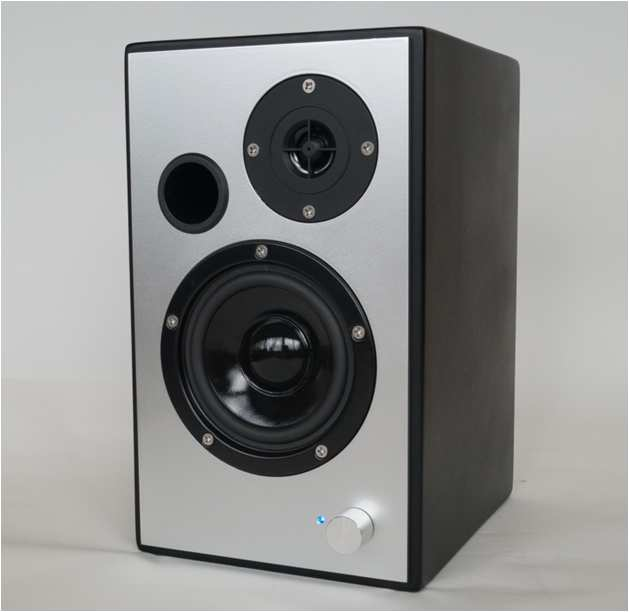
\includegraphics[width=\textwidth]{images/upone0}
        \graphicscaption{Schlichtes Design des UPone}
    \end{minipage}
    \begin{minipage}{0.4\textwidth}
        \centering
        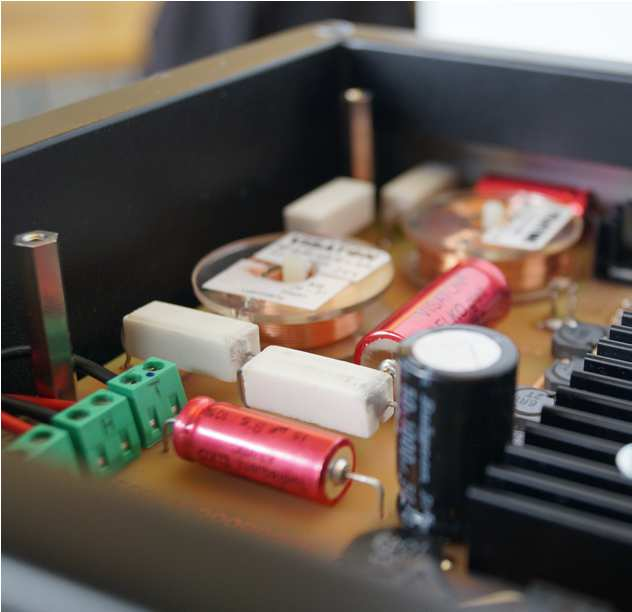
\includegraphics[width=\textwidth]{images/upone1}
        \graphicscaption{modernste Technik, kompakt verpackt.}
    \end{minipage}
}

\fscontent{
    \section{Die Aufgabe}
    Die   heutigen  Wiedergabegeräte   sind   teuer   oder  haben   schlechte
    Qualität. Dabei   spielen  teure   Herstellerzertifikate  und   schlechte
    Materialwahl  eine  Rolle.   Der  UPone  stellt  die  Lösung  für  diese
    beiden Probleme. Der  Lautsprecher kann  Mittels DLNA Musik  empfangen und
    wiedergeben. Mit dem  2-Weg-System, bestehendend aus einem  Hochtöner und
    einem Tiefmitteltöner wird eine ausgezeichnete Klangqualität erreicht.

    \section{Das Geh\"ause}
    Das Gehäuse, welches komplett aus Holz  besteht, hat ein Volumen von vier
    Liter. Im Gehäuse ist zusätzlich  ein Bassreflexrohr angebracht, welches
    für  einen  kräftigeren Bass  im  gewählten  Song sorgt. Ein  schwarzes
    Gehäuse  mit einer  mattpolierten Aluplatte  gibt dem  UPone die  nötige
    Schlichtheit aber auch Eleganz.

    \section{Die Technik}
    Der  UPone  besitzt  ein hochstehendes  Innenleben. Das  Herzstück  dabei
    bildet das Raspberry  Pi, ein Mini Computer  mit Linux Betriebssystem. Das
    Raspberry  Pi sorgt  dabei für  die  Kommunikation mit  dem Netzwerk  und
    Wiedergabe der Musik.  Zudem besitzt  der UPone einen Klass D Verstärker,
    welcher das Audiosignal in ausgezeichneter Qualität den zwei Lautsprecher
    bereitstellt.    Der  Lautsprecher   besitzt  eine   Ausgangsleistung  von
    \SI{30}{\watt} einen  mittleren Schaldruck von \SI{82}{\dB}  und einen THD
    von \SI{3.5}{\percent}. Der Standby-Verbrauch liegt bei \SI{7.5}{\watt}.

    \section{Die Handhabung}
    Der  UPone ist  für  den  Kunden einfach  zu  bedienen.   Durch die  Push
    Button Konfiguration  kann der  UPone einfach  mit einem  gesicherten WLAN
    verbunden  werden.  Eine  dezente blaue  LED an  der Frontseite  zeigt dem
    Benutzer die Stromversorgung an.  Die Bedienung selbst erfolgt über einen
    modernen  metallene  Drehschalter,  welcher  als  Powerschalter  fungiert,
    wie  auch als  Lautstärkeregelung  Auf der  Rückseite  sind Line-In  wie
    auch Line-Out \SI{3.5}{\mm}-Klinken-Anschlüsse. Somit  kann der UPone als
    normaler Lautsprecher oder als Verstärker betrieben werden.
}

\infobox{Die Qual der Wahl}{%
    \begin{minipage}[t][][b]{0.45\textwidth}
        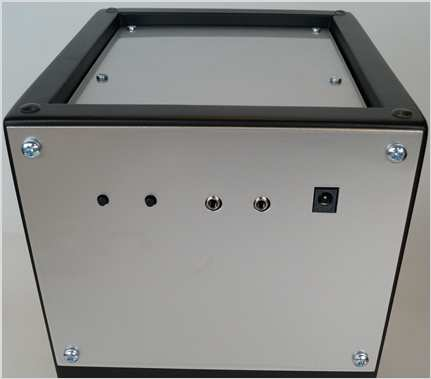
\includegraphics[width=\textwidth]{images/upone2}
    \end{minipage}
    \hfill
    \begin{minipage}[t][][b]{0.50\textwidth}\small
        Der UPone kann  über WLAN oder durch den  Line-In Anschluss betrieben
        werden,   mit dem  PC, Smartphone,  MP3 Player  oder direkt  von einem
        Verstärker.
    \end{minipage}
}
